% GNUPLOT: LaTeX picture with Postscript
\begingroup
  \makeatletter
  \providecommand\color[2][]{%
    \GenericError{(gnuplot) \space\space\space\@spaces}{%
      Package color not loaded in conjunction with
      terminal option `colourtext'%
    }{See the gnuplot documentation for explanation.%
    }{Either use 'blacktext' in gnuplot or load the package
      color.sty in LaTeX.}%
    \renewcommand\color[2][]{}%
  }%
  \providecommand\includegraphics[2][]{%
    \GenericError{(gnuplot) \space\space\space\@spaces}{%
      Package graphicx or graphics not loaded%
    }{See the gnuplot documentation for explanation.%
    }{The gnuplot epslatex terminal needs graphicx.sty or graphics.sty.}%
    \renewcommand\includegraphics[2][]{}%
  }%
  \providecommand\rotatebox[2]{#2}%
  \@ifundefined{ifGPcolor}{%
    \newif\ifGPcolor
    \GPcolortrue
  }{}%
  \@ifundefined{ifGPblacktext}{%
    \newif\ifGPblacktext
    \GPblacktexttrue
  }{}%
  % define a \g@addto@macro without @ in the name:
  \let\gplgaddtomacro\g@addto@macro
  % define empty templates for all commands taking text:
  \gdef\gplbacktext{}%
  \gdef\gplfronttext{}%
  \makeatother
  \ifGPblacktext
    % no textcolor at all
    \def\colorrgb#1{}%
    \def\colorgray#1{}%
  \else
    % gray or color?
    \ifGPcolor
      \def\colorrgb#1{\color[rgb]{#1}}%
      \def\colorgray#1{\color[gray]{#1}}%
      \expandafter\def\csname LTw\endcsname{\color{white}}%
      \expandafter\def\csname LTb\endcsname{\color{black}}%
      \expandafter\def\csname LTa\endcsname{\color{black}}%
      \expandafter\def\csname LT0\endcsname{\color[rgb]{1,0,0}}%
      \expandafter\def\csname LT1\endcsname{\color[rgb]{0,1,0}}%
      \expandafter\def\csname LT2\endcsname{\color[rgb]{0,0,1}}%
      \expandafter\def\csname LT3\endcsname{\color[rgb]{1,0,1}}%
      \expandafter\def\csname LT4\endcsname{\color[rgb]{0,1,1}}%
      \expandafter\def\csname LT5\endcsname{\color[rgb]{1,1,0}}%
      \expandafter\def\csname LT6\endcsname{\color[rgb]{0,0,0}}%
      \expandafter\def\csname LT7\endcsname{\color[rgb]{1,0.3,0}}%
      \expandafter\def\csname LT8\endcsname{\color[rgb]{0.5,0.5,0.5}}%
    \else
      % gray
      \def\colorrgb#1{\color{black}}%
      \def\colorgray#1{\color[gray]{#1}}%
      \expandafter\def\csname LTw\endcsname{\color{white}}%
      \expandafter\def\csname LTb\endcsname{\color{black}}%
      \expandafter\def\csname LTa\endcsname{\color{black}}%
      \expandafter\def\csname LT0\endcsname{\color{black}}%
      \expandafter\def\csname LT1\endcsname{\color{black}}%
      \expandafter\def\csname LT2\endcsname{\color{black}}%
      \expandafter\def\csname LT3\endcsname{\color{black}}%
      \expandafter\def\csname LT4\endcsname{\color{black}}%
      \expandafter\def\csname LT5\endcsname{\color{black}}%
      \expandafter\def\csname LT6\endcsname{\color{black}}%
      \expandafter\def\csname LT7\endcsname{\color{black}}%
      \expandafter\def\csname LT8\endcsname{\color{black}}%
    \fi
  \fi
    \setlength{\unitlength}{0.0500bp}%
    \ifx\gptboxheight\undefined%
      \newlength{\gptboxheight}%
      \newlength{\gptboxwidth}%
      \newsavebox{\gptboxtext}%
    \fi%
    \setlength{\fboxrule}{0.5pt}%
    \setlength{\fboxsep}{1pt}%
\begin{picture}(7200.00,5040.00)%
    \gplgaddtomacro\gplbacktext{%
      \colorrgb{0.15,0.15,0.15}%%
      \put(804,2942){\makebox(0,0)[r]{\strut{}0}}%
      \colorrgb{0.15,0.15,0.15}%%
      \put(804,3157){\makebox(0,0)[r]{\strut{}1000}}%
      \colorrgb{0.15,0.15,0.15}%%
      \put(804,3372){\makebox(0,0)[r]{\strut{}2000}}%
      \colorrgb{0.15,0.15,0.15}%%
      \put(804,3587){\makebox(0,0)[r]{\strut{}3000}}%
      \colorrgb{0.15,0.15,0.15}%%
      \put(804,3802){\makebox(0,0)[r]{\strut{}4000}}%
      \colorrgb{0.15,0.15,0.15}%%
      \put(804,4016){\makebox(0,0)[r]{\strut{}5000}}%
      \colorrgb{0.15,0.15,0.15}%%
      \put(804,4231){\makebox(0,0)[r]{\strut{}6000}}%
      \colorrgb{0.15,0.15,0.15}%%
      \put(804,4446){\makebox(0,0)[r]{\strut{}7000}}%
      \colorrgb{0.15,0.15,0.15}%%
      \put(804,4661){\makebox(0,0)[r]{\strut{}8000}}%
      \colorrgb{0.15,0.15,0.15}%%
      \put(2052,2722){\makebox(0,0){\strut{}Proteins}}%
      \colorrgb{0.15,0.15,0.15}%%
      \put(3168,2722){\makebox(0,0){\strut{}Carbohydrates}}%
      \colorrgb{0.15,0.15,0.15}%%
      \put(4283,2722){\makebox(0,0){\strut{}Fats}}%
      \colorrgb{0.15,0.15,0.15}%%
      \put(5399,2722){\makebox(0,0){\strut{}Fibers}}%
    }%
    \gplgaddtomacro\gplfronttext{%
      \csname LTb\endcsname%%
      \put(67,3801){\rotatebox{-270}{\makebox(0,0){\strut{}Nutritional Value}}}%
      \put(3725,2392){\makebox(0,0){\strut{}Macro Nutrient Name}}%
      \csname LTb\endcsname%%
      \put(5987,4488){\makebox(0,0)[l]{\strut{}LB}}%
      \csname LTb\endcsname%%
      \put(5987,4268){\makebox(0,0)[l]{\strut{}LB}}%
      \csname LTb\endcsname%%
      \put(5987,4048){\makebox(0,0)[l]{\strut{}LB}}%
    }%
    \gplgaddtomacro\gplbacktext{%
      \colorrgb{0.15,0.15,0.15}%%
      \put(804,554){\makebox(0,0)[r]{\strut{}0}}%
      \colorrgb{0.15,0.15,0.15}%%
      \put(804,769){\makebox(0,0)[r]{\strut{}10000}}%
      \colorrgb{0.15,0.15,0.15}%%
      \put(804,984){\makebox(0,0)[r]{\strut{}20000}}%
      \colorrgb{0.15,0.15,0.15}%%
      \put(804,1199){\makebox(0,0)[r]{\strut{}30000}}%
      \colorrgb{0.15,0.15,0.15}%%
      \put(804,1414){\makebox(0,0)[r]{\strut{}40000}}%
      \colorrgb{0.15,0.15,0.15}%%
      \put(804,1628){\makebox(0,0)[r]{\strut{}50000}}%
      \colorrgb{0.15,0.15,0.15}%%
      \put(804,1843){\makebox(0,0)[r]{\strut{}60000}}%
      \colorrgb{0.15,0.15,0.15}%%
      \put(804,2058){\makebox(0,0)[r]{\strut{}70000}}%
      \colorrgb{0.15,0.15,0.15}%%
      \put(804,2273){\makebox(0,0)[r]{\strut{}80000}}%
      \colorrgb{0.15,0.15,0.15}%%
      \put(1733,334){\makebox(0,0){\strut{}Calcium}}%
      \colorrgb{0.15,0.15,0.15}%%
      \put(2530,334){\makebox(0,0){\strut{}Magnesio}}%
      \colorrgb{0.15,0.15,0.15}%%
      \put(3327,334){\makebox(0,0){\strut{}Fosfer}}%
      \colorrgb{0.15,0.15,0.15}%%
      \put(4124,334){\makebox(0,0){\strut{}Ferro}}%
      \colorrgb{0.15,0.15,0.15}%%
      \put(4921,334){\makebox(0,0){\strut{}Zinc}}%
      \colorrgb{0.15,0.15,0.15}%%
      \put(5718,334){\makebox(0,0){\strut{}Manganes}}%
    }%
    \gplgaddtomacro\gplfronttext{%
      \csname LTb\endcsname%%
      \put(-65,1413){\rotatebox{-270}{\makebox(0,0){\strut{}Nutritional Value}}}%
      \put(3725,4){\makebox(0,0){\strut{}Micro nutrient Name}}%
      \csname LTb\endcsname%%
      \put(5987,2100){\makebox(0,0)[l]{\strut{}LB}}%
      \csname LTb\endcsname%%
      \put(5987,1880){\makebox(0,0)[l]{\strut{}LB}}%
      \csname LTb\endcsname%%
      \put(5987,1660){\makebox(0,0)[l]{\strut{}LB}}%
    }%
    \gplbacktext
    \put(0,0){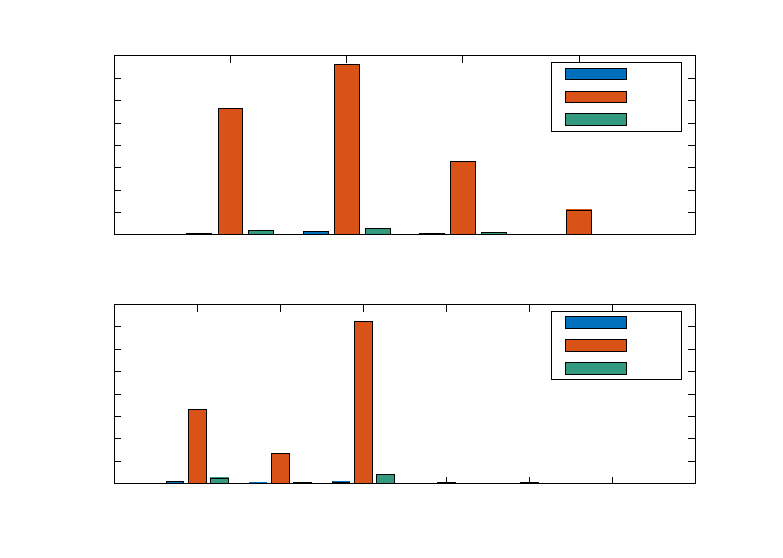
\includegraphics{/home/glauber/CLionProjects/modern-nutrition/exports/nutritional-menu-result/nutrients-latex}}%
    \gplfronttext
  \end{picture}%
\endgroup
